\documentclass[svgnames]{article}   	% use "amsart" instead of "article" for AMSLaTeX format
%\geometry{landscape}                	% Activate for rotated page geometry

%\usepackage[parfill]{parskip}    		% Activate to begin paragraphs with an empty line rather than an indent

\usepackage{graphicx}				          % Use pdf, png, jpg, or eps§ with pdflatex; use eps in DVI mode

%maths							                  % TeX will automatically convert eps --> pdf in pdflatex		
\usepackage{amssymb}
\usepackage{amsmath}
\usepackage{esint}
\usepackage{geometry}

%pgfplots
\usepackage{pgfplots}

%images
\graphicspath{{/Users/devaldeliwala}}					          % Activate to set a image directory 

%tikz
\usepackage{pgfplots}
\pgfplotsset{compat=1.15}
\usepackage{comment}
\usetikzlibrary{arrows}

%Figures
\usepackage{float}
\usepackage{caption}
\usepackage{lipsum}
\usepackage[most]{tcolorbox}



\title{Introduction to Quantum Mechanics}
\author{deval deliwala}
%\date{}							                % Activate to display a given date or no date

\begin{document}
\maketitle
\begin{center}
Adapted from \textit{Introduction to Quantum Mechanics} 3rd ed. By David J.
Griffiths
\end{center}


\vspace{20px} \vspace{20px}
\begin{center}
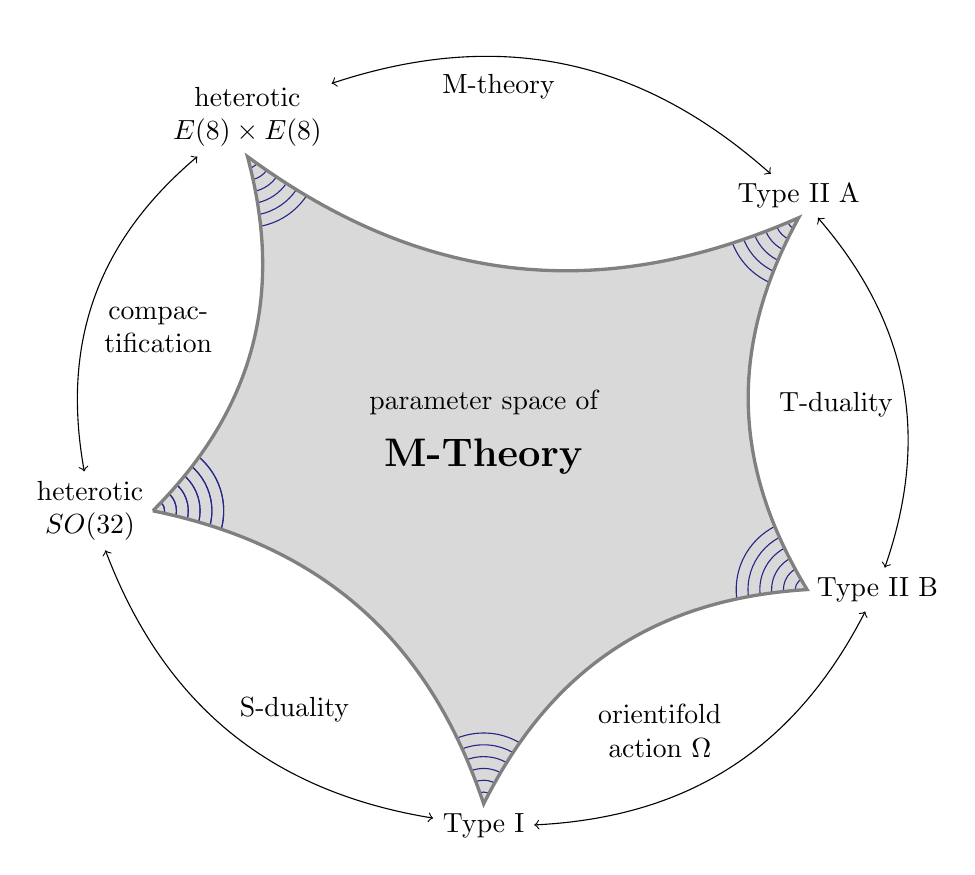
\begin{tikzpicture}

  \node (so32) [align=center] at (-5,-1) {heterotic\\$SO(32)$};
  \node (e8e8) [align=center] at (-3,4) {heterotic\\$E(8) \times E(8)$};
  \node (tiia) [align=center] at (4,3) {Type II A};
  \node (tiib) [align=center] at (5,-2) {Type II B};
  \node (ti) [align=center] at (0,-5) {Type I};

  \draw[bend left,<->] (so32) to node [below right,align=center] {compac-\\tification} (e8e8);
  \draw[bend left,<->] (e8e8) to node [below left] {M-theory} (tiia);
  \draw[bend left,<->] (tiia) to node [below left] {T-duality} (tiib);
  \draw[bend left,<->] (tiib) to node [above left,align=center] {orientifold\\action $\Omega$} (ti);
  \draw[bend left,<->] (ti) to node [above right] {S-duality} (so32);

  \begin{scope}
    \clip[bend right]
    (so32.east)
    to (e8e8.south)
    to (tiia.south)
    to (tiib.west)
    to (ti.north)
    to (so32.east);
    \foreach \c in {so32.east,e8e8.south,tiia.south,tiib.west,ti.north,so32.east}{%
        \foreach \r in {1,...,6}{%
            \draw[DarkBlue] (\c) circle (\r*0.15cm);
          }
      }
  \end{scope}

  \draw[bend right,very thick,gray,fill,fill opacity=0.3] (so32.east) to (e8e8.south) to (tiia.south) to (tiib.west) to (ti.north) to (so32.east);

  \node (mth) [align=center] at (0,0) {parameter space of\\[2ex]{\Large \textbf{M-Theory}}};

\end{tikzpicture}
\end{center}

\newpage
\tableofcontents
\newpage

\section{The Wave Function}

\subsection{The Schr\"{o}dinger Equation} \mbox{}\\

Imagine a particle of mass $m$, constrained to move along the $x$ axis, subject
to move to some specified force $F(x,t)$. The program of \textit{classical
mechanics} is to determine the position of the particle at any given time
$x(t)$. Once we know that, we can figure out the velocity $(v
= \frac{dx}{dt})$, the momentum $p = mv$, the kinetic energy $(T = \frac{1}{2}mv^2)$,
or any other dynamical variable of interest. To determine $x(t)$, we apply
Newton's Second Law: $F = ma$, or more specifically, $F = -\frac{\partial
V}{\partial x}$, the derivative of a potential energy function, where
$m\frac{\partial^2 x}{\partial t^2} = - \frac{\partial V}{\partial x}$. This
together, with initial conditions, determines $x(t)$. \\\\
Quantum mechanics approaches this same problem a bit differently. In this case
what we're looking for is the particles \textbf{wave function}, $\Phi(x,t)$,
and we get it by solving the \textbf{Schr\"{o}dinger Equation:} 
\\
\begin{tcolorbox}[colback = red!5!white, colframe = red!50!black, title
  = Schr\"{o}dinger Equation]

  \[
  i\hbar\frac{\partial \Psi}{\partial t} = - \frac{\hbar^2}{2m}\frac{\partial^2
  \Phi}{\partial x^2} + V\Phi
  \] 

\end{tcolorbox} \mbox{}\\


Here $i$ is the square root of $-1$, and $\hbar$ is Planck's constant - or
rather, his \textit{original} constant $(h)$ divided by  $2\pi$: 

\[
  \hbar = \frac{h}{2\pi} = 1.054573 \times 10^{-34} J s. 
\] \\

The Schr\"{o}dinger equation plays a role logically analogous to Newton's
second law. \\

\subsection{The Statistical Interpretation} \mbox{}\\


But what exactly \textit{is} this wave function, and what does it do for you
once you've \textit{got} it? After all a particle by nature is a point, whereas
the wave function (as its name suggests) is spread out in space (a function of
$x$, for any given  $t$). 

\begin{figure}[htb!]
  \centering
  \includegraphics[width = 10cm]{screenshot 12.png}
    \caption{a "particle" constrained to move in one dimension under the
    influence of a specified force}
\end{figure}

\begin{figure}[htb!]
  \centering
  \includegraphics[width = 10cm]{screenshot 13.png}
    \caption{a typical wave function. the shaded area represents the
    probability of finding the particle between $a$ and $b$. the particle would
  be relatively likely to be found near  $A$, and unlikely to be found near
$B$.}
\end{figure} 



How can such an object represent the state of a \textit{particle}? The answer
is provided by Born's \textbf{statistical interpretation}, which says that
$|\Psi(x,t)|^2$ gives the \textit{probability} of finding the particle at point
$x$, at time $t$ - or, more precisely, 
\\

\begin{tcolorbox}[colback = blue!5!white, colframe = blue!50!black, title
  = Born's Statistical Interpretation]
\[  
\int_{a}^{b} |\Psi(x,t)|^2\,dx = \{ \text{probability of finding particle
between $a$ and $b$, at time $t$ }\} 
\]
\end{tcolorbox} \mbox{}\\

Probability is the \textit{area} under the graph of $|\Psi|^2$. For the wave
function in the figure above, you would be quite likely to find the particle in
the vicinity of point A, where $|\Psi|^2$ is large, and relatively unlikely to
find it near point $B$. \\ \\ 

The statistical interpretation introduces a kind of \textbf{indeterminacy} into
quantum mechanics, for even if you know everything, the theory has to tell you
about the particle, still you can't predict with certainty the outcome of
a simple experiment to predict its position - all quantum mechanics has to
offer is \textit{statistical} information about \textit{possible} results. It
is natural to wonder whether this indeterminacy is a fact of nature, or
a defect in the theory. \\\\

Suppose I \textit{do} measure the position of the particle, and I find it to be
a point $C$. \mbox{}\\ \\

\textbf{\textit{Question}}\\\\
Where was the particle just  \textit{before} I made the measurement? \\\\

\textbf{\textit{Solution}}\\\\
There are three plausible answers \vspace{5px}

\begin{tcolorbox}	
  
  1. The \textbf{realist} position: The \textit{particle was at} $C$. This
     certainly seems reasonable, and it is the response Einstein advocated.
     However, if this is true, quantum mechanics is an \textit{incomplete}
     theory, since the particle \textit{really was} at $C$, and yet quantum
     mechanics was unable to tell us so. 

\end{tcolorbox} \vspace{5px}

\begin{tcolorbox}	
  
  2. The \textbf{orthodox} position: The \textit{particle wasn't really
anywhere}. It was the act of measurement that forced it to "take a stand"
(though how and why it chose the point $C$ we dare not ask). This view is
associated with Bohr and his followers. Among physicists it is the most widely
accepted position. However, if it is correct, a century worth of debate about
the act of measurement has done preciously little to illuminate. 

\end{tcolorbox}	\vspace{5px}

\begin{tcolorbox}	
  
  The \textbf{agnostic} position: \textit{Refuse to answer}. This is not as
  silly as it sounds - what sense can there be in making assertions about the
  status of a particle \textit{before} a measurement. For decades this was the
  "fall-back" position of most physicists: they'd try to sell you the orthodox
  answer, but if you were persistent they'd retreat to the agnostic response,
  and terminate the conversation.

\end{tcolorbox} \vspace{20px}	

However, in 1964, John Bell astonished the physics community by showing that it
makes an \textit{observable} difference whether the particle had a precise
(though unknown) position prior to the measurement or not. Bell's discovery
effectively eliminated agnosticism as a viable option and made it an
\textit{experimental} question whether 1 or 2 was the correct choice. \\\\

What if I made a \textit{second} measurement, immediately after the first?
Would I get $C$ again, or does the act of measurement cough up a completely new
number each time? On this question everyone is in agreement: 

\[
\text{A repeated measurement (on the same particle) must return the same
value}    
\]\\

Indeed, it would be tough to prove the particle was really at $C$ in the first
instance. How does the orthodox interpretation account for the fact that the
second measurement is bound to yield the same result $C$? It must be that the
first measurement radically alters the wave function, so that it now sharply
peaked about $C$. We say that a wave function \textbf{collapses}, upon
measurement, to a spike at the point $C$ (it soon spreads out again, in
accordance with the Schr\"{o}dinger equation, so the second measurement must be
made quickly). 
\vspace{20px}
\begin{figure}[hb!]
  \centering
    \includegraphics[width = 10cm]{screenshot 14.png}
    \caption{collapse of the wave function: graph of $|\Psi|^2$ immediately
    \textit{after} a measurement has found the particle at point $C$.}
\end{figure}
\vspace{20px}
There are then, two entirely distinct kinds of physical processes: "ordinary"
ones, in which the wave function evolves in a leisurely fashion under the
Schr\"{o}dinger equation, and "measurements," in which $\Psi$ suddenly and
discontinuously collapses. 


\subsubsection{Example 1.1} \mbox{}\\

\textbf{Electron Interference}. How might we check that particles (electrons,
for example) have a wave nature, encoded in $\Psi$? \\\\
The classic signature of a wave phenomena is \textit{interference}: two waves
\textit{in phase} interfere constructively, and out of phase they interfere
destructively. The wave nature of light wave confirmed in 1801 by Young's
famous double slit experiment, showing interference "fringes" on a distant
screen when a monochromatic beam passes through two slits. If essentially the
same experiment is done with \textit{electrons}, the same pattern develops,
confirming the wave nature of electrons as more and more electrons collide with
the screen. 

\begin{figure}[hb!]
  \centering
    \includegraphics[width = 5.5cm]{screenshot 15.png}
    \caption{Build up of electron interference pattern. (a) Eight electrons,
    (b) 270 electrons, (c) 2000 electrons, (d) 160,000 electrons.}
\end{figure}
Of course, if you close off one slit, or somehow contrive to detect which slit
each electron passes through, the interference pattern disappears; the wave
function of the emerging particle is now entirely different.

\vspace{20px}
\section{Probability}
\subsection{Discrete Variables}
\vspace{20px}

Because of statistical interpretation, probability plays a central role in
quantum mechanics, so I digress now for a brief discussion of probability
theory. It is mainly a question of introducing some notation and terminology,
and I shall do it in the context of a simple example: \\\\

Imagine a room containing 14 people, whose ages are: \\\\

\noindent one person aged 14\\
one person aged 15\\
three people aged 16\\
two people aged 22\\
two people aged 24\\
five people aged 25\\\\

If we let $N(j)$ represent the number of people of age $j$, then \\\\
$
N(14) = 1 \\
N(15) = 1 \\
N(16) = 3 \\
N(22) = 2 \\
N(24) = 2 \\
N(25) = 5 \\ \\ 
$
\begin{figure}[htb!]
  \centering
    \includegraphics[width = 10cm]{screenshot 16.png}
    \caption{histogram of people}
\end{figure}

while $N(17)$, for instance, is 0. The total number of people in the room is 

\vspace{5px}\[
  N = \sum_{j=0}^{\infty} N(j). 
\] \vspace{5px}


\textbf{\textit{Question}} \vspace{10px} 
If you selected one individual at random from this group, what is the
\textbf{probability} that this person's age would be 15? \vspace{10px}
\textbf{\textit{Solution}} \vspace{10px}
One chance in 14, since there are 14 possible choices, all equally likely, of
whom only one is aged 14. If $P(j)$ is the probability of getting age $j$,
then $P(14) = 1/14, P(15) = 1/14, P(16) = 3/14$, and so one. In general, 

\vspace{5px}\[
P(j) = \frac{N(j)}{N}.
\] \vspace{5px} 

Notice that the probability of getting \textit{either} 14 or 15 is the
\textit{sum} of the individual probabilities (1/7). In particular, the sum of
\textit{all} probabilities is 1 - the person you select must have \textit{some}
age: 

\vspace{5px} \[
\sum_{j=0}^{\infty} P(j) =1
\] \vspace{5px}

\begin{tcolorbox}[colback = blue!5!white, colframe = blue!50!black, title
= Question]
What is the \textbf{most probable} age? 
\end{tcolorbox} 

\begin{tcolorbox}[colback = red!5!white, colframe = red!50!black, title
= Solution]
25, obviously, the most probably $j$ is the $j$ for which $P(j)$ is a maximum. 
\end{tcolorbox} 

\begin{tcolorbox}[colback = blue!5!white, colframe = blue!50!black, title
= Question]
What is the \textbf{median} age?   
\end{tcolorbox} 

\begin{tcolorbox}[colback = red!5!white, colframe = red!50!black, title
= Solution]
23, for 7 people are younger than 23, and 7 people are older  
\end{tcolorbox} 

\begin{tcolorbox}[colback = blue!5!white, colframe = blue!50!black, title
= Question]
What is the \textbf{median} age?
\end{tcolorbox} 

\begin{tcolorbox}[colback = red!5!white, colframe = red!50!black, title
= Solution]
\[
\frac{14 + 15 + 3(16) + 2(22) + 2(24) + 5(25)}{14} = \frac{294}{14} = 21.
\]

\end{tcolorbox}

\vspace{5px}
In general, the average value of $j$, which we will write as $\langle
j \rangle$ is 

\vspace{5px} \[
  \langle j \rangle = \frac{\sum j N(j)}{N} = \sum_{j=0}^{\infty} j P(j). 
\] \vspace{5px}

In quantum mechanics the average is usually the quantity of interest; it is
known as the \textbf{expectation value}. \\[0.5cm]

\begin{tcolorbox}[colback = blue!5!white, colframe = blue!50!black, title
= Question]
What is the average of the \textit{squares} of the ages? 
\end{tcolorbox} \

\begin{tcolorbox}[colback = red!5!white, colframe = red!50!black, title
= Solution]
You could get $14^2 = 196$ with probability 1/14, or $15^2 = 225$, with
probability 1/14, or $16^2 = 256$ with probability 3/14, and so on. The average
is then 

\[
  \langle j^2 \rangle = \sum_{j=0}^{\infty} j^2 P(j) 
\]

\end{tcolorbox} \vspace{5px}

In general, the average value of some \textit{function} of $j$ is given by
\vspace{5px}
\begin{tcolorbox}	
 \[ 
  \langle f(j) \rangle = \sum_{j=0}^{\infty} f(j)P(j). 
  \]
\end{tcolorbox}	

\vspace{5px}

\textit{Beware:} The average of the squares, $\langle j^2 \rangle$, is
\textit{not} equal, in general, to the square of the average, $\langle
j \rangle ^2$. 
\vspace{5px}

\begin{figure}[htb!]
  \centering
    \includegraphics[width = 10cm]{screenshot 17.png}
    \caption{two histograms with the same median, mean, and same most probable
    value, but different standard deviations}
\end{figure}

\vspace{5px}

Now, there is a difference between the two histograms. The first is sharply
peaked about the average, with the same number of elements, whereas the second
is broad and flat. We need a numerical measure of the amount of "spread" in
a distribution, with respect to the average. To get a value we can work with,
we also square the value before average
\vspace{5px} \[
\sigma^2 \equiv \langle (\Delta j)^2 \rangle.
\] \vspace{5px}
This quantity is known as the \textbf{variance} of the distribution; $\sigma$
itself is called the \textbf{standard deviation}, which measures the spread
about $\langle j \rangle$. Taking the square root, the standard deviation can
be written as 

\vspace{5px} \[
\sigma = \sqrt{\langle j^2\rangle - \langle j \rangle ^2}  
\] \vspace{5px}

\subsection{Continuous Variables}

So far we've only dealt with specific variables, not continuous and more
realistic ones. The sensible thing to speak about is the probability of
a variable existing in some \textit{interval} - say, between 16 and 17 years
old in the previous example. If the interval is sufficiently short, this
probability is \textit{proportional to the length of the interval}.
Technically, we're talking about \textit{infinitesimal} intervals. 

\vspace{5px} \[
  \{ \text{probability that an individual lies between $x$ and  $(x + dx)$ \}}
    = \rho(x) \,dx . 
\] \vspace{5px}


More specifically, the proportionality factor, $\rho(x)$ is better defined as
\textbf{probability density}. The probability that $x$ lies between $a$ and $b$
is given by the integral of $\rho(x)$ : 

\vspace{5px} \[
  P_{ab} = \int_{a}^{b} \rho(x) \, dx,  
\] \vspace{5px}

and the rules we deduced for discrete distributions translate in the obvious
way: 

\begin{align*}
  \int_{-\infty}^{\infty} \rho(x) \, dx = 1 \\
  \langle x \rangle = \int_{-\infty}^{\infty}  x\rho(x)\,dx, \\
  \langle f(x) \rangle = \int_{-\infty}^{\infty}  f(x) \rho(x) \, dx, \\
  \sigma^2 \equiv \langle ( \Delta x)^2 \rangle = \langle x^2 \rangle - \langle
  x \rangle ^2
\end{align*}


\subsubsection{Example 1.2}

Suppose someone drops a rock off a cliff of height $h$. As it falls, I snap
a million photographs at random intervals. On each picture I measure the
distance the rock has fallen. \\

\begin{tcolorbox}[colback = blue!5!white, colframe = blue!50!black, title
= Question]
What is the \textit{average} of all these distances, or rather the \textit{time
average} of the distance traveled? 
\end{tcolorbox} 

\begin{tcolorbox}[colback = red!5!white, colframe = red!50!black, title
= Solution]
The rock starts out at rest, then falls so 

\[
x(t) = \frac{1}{2}gt^2
\]

The velocity is $dx/dt= gt$ and the total flight time is $T = \sqrt{2h/g}$. The
probability that a particular photograph was taken between $t$ and $t + dt$ is
$dt / T$, so the probability that is shows a distance in the range $x$ to $x
+ dx$ is 

\[
  \frac{dt}{T} = \frac{dx}{gt}\sqrt{\frac{g}{2h}} = \frac{1}{2\sqrt{hx}}dx. 
\]

Thus the probability \textit{density} is 

\[
  \rho(x) = \frac{1}{2\sqrt{hx}}, \hspace{10px} (0 \leq x \leq h)
\]

We can check this result, 

\[
  \int_{0}^{h} \rho(x)\,dx = \frac{1}{2\sqrt{h}}(2x^{1/2}) \Big|_0^h = 1 
\]

The \textit{average} distance is 
\[
  \langle x \rangle = \int_{0}^{h} x\frac{1}{2\sqrt{hx}} \,dx
  = \frac{1}{2\sqrt{h}} (\frac{2}{3}x^{3/2})\Big|_0^h = \frac{h}{3}, 
\]

which is somewhat less than $h/2$, as anticipated. The image below shows the
graph of $\rho(x)$, notice that the probability density can be infinite, though
the probability itself must of course be finite, less than or equal to 1. 


\end{tcolorbox} 


\begin{figure}[htb!]
  \centering
    \includegraphics[width = 7cm]{screenshot 18.png}
    \caption{the probability density: $\rho(x) = 1/(2\sqrt{hx})$}
\end{figure}


\subsubsection{Problem 1.1} For the distribution of ages in the example above: 

\begin{tcolorbox}	
  
  (a) Compute $\langle j^2 \rangle$ and $\langle j \rangle^2$ \\
  (b) Determine $\Delta j$ for each $j$ and compute the standard deviation\\
  (c) Use your results in (a) and (b) to check if the standard deviation makes sense. 
  
\end{tcolorbox}	


\begin{figure}[H]
  \centering
    \includegraphics[width = 17cm]{screenshot 22.png}
    \caption{solutions for problem 1.1}
\end{figure}


\subsubsection{Problem 1.2} 

\begin{tcolorbox}	
  
(a) Find the standard deviation of the distribution in Example 1.2\\
(b) What is the probability that a photograph, selected at random, would show
a distance $x$ more than one standard deviation away from the average?

\end{tcolorbox}	

\begin{figure}[H]
  \centering
    \includegraphics[width = 17cm]{screenshot 20.png}
    \caption{solutions to problem 1.2}
\end{figure}

\subsubsection{Problem 1.3} Consider the \textbf{gaussian} distribution 

\vspace{5px} \[
  \rho(x) = Ae^{-\lambda (x-a)^2}, 
\] \vspace{5px}

where $A, a$ and  $\lambda$ are positive real constants. 

\begin{tcolorbox}	
  
  (a) Use the fact that $\int \rho(x) \, dx = 1$ to determine  $A$ \\
  (b) Find $\langle x \rangle, \langle x^2 \rangle$ and $\sigma$ \\
  (c) Sketch $\rho(x)$

\end{tcolorbox}	

\begin{figure}[H]
  \centering
    \includegraphics[width = 17cm]{screenshot 21.png}
    \caption{solution to problem 1.3}
\end{figure}

\section{Normalization}

We now return to the statistical interpretation of the wave function, which
says that $|\Psi(x,t)|^2$ is the probability density for finding the particle
at point $x$ at time $t$. Therefore, i
\vspace{5px}
\begin{tcolorbox}	
  \[
  \int_{-\infty}^{\infty} |\Psi(x,t)|^2 \, dx = 1 
  \]
\end{tcolorbox}	
\vspace{5px}

However, $\Psi(x,t)$ must also be a solution to the Schrodinger equation, as
that is how it is determined. A glance at the Schrodinger equation reveals that
if $\Psi(x,t)$ is a solution, so too is $A\Psi(x,t)$, where A is any
(complex)constant. This process of finding a constant $A$ such that $\Psi(x,t)$
satisfies both the above integral and Schrodinger's Equation is known as
\textbf{normalizing} the wave function. 
\vspace{5px}
For some solutions to the Schrodinger equation, the integral above is infinite,
in that case there exists no $A$ that would make it 1. The same goes for the
trivial solution $\Psi = 0$. Such \textbf{non-normalizable} solutions cannot
represent particles, and are therefore rejected. Physically realizable states
correspond to the \textbf{square-integrable} solutions to Schrodinger's
Equation. 
\vspace{5px}
But wait!. Suppose I have normalized the wave function at time $t=0$. How do
I know it will \textit{stay} normalized as time goes on, and $\Psi$ evolves?
Fortunately Schrodinger's Equation has the remarkable property that it
\textit{preserves} the normalization of a wave function. 
\vspace{5px}

This is important, so let us prove it. 


\vspace{20px}
\noindent\textbf{\textit{Proof}} 
  \[
  \frac{d}{dt} \int_{-\infty}^{\infty}  |\Psi(x,t)|^2 \, dx
  = \int_{-\infty}^{\infty}  \frac{\partial}{\partial t} |\Psi(x,t)|^2 \, dx  
  \] 
 *Note that the integral is only a function of $t$, so a normal derivative
 works. The integrand is a function of both $x,t$ so we use a partial
 derivative. 
 \vspace{5px}
 By the product rule, 

 \[
 \frac{\partial}{\partial t} |\Psi|^2 = \frac{\partial}{\partial t}(\bar\Psi
 \Psi) = \bar\Psi \frac{\partial \Psi}{\partial t} + \frac{\partial
 \bar\Psi}{\partial t}\Psi
 \vspace{5px}
 \]
 Now the Schrodinger equation says that 

 \[
 \frac{\partial \Psi}{\partial t} = \frac{i \hbar}{2m}\frac{\partial^2
 \Psi}{\partial x^2} - \frac{i}{\hbar}V\Psi
 \]
 \vspace{5px}
 and hence also (taking complex conjugate)

 \[
   \frac{\partial \bar\Psi}{\partial t} = \frac{i\hbar}{2m} \frac{\partial^2
  \bar\Psi}{\partial x^2} - \frac{i}{\hbar}V\bar\Psi  
 \]
 \vspace{5px}
 so 

 \vspace{5px} \[
 \frac{\partial }{\partial t} |\Psi|^2 = \frac{i\hbar}{2m}\left(\bar\Psi
   \frac{\partial^2 \Psi}{\partial x^2} - \frac{\partial^2 \bar\Psi}{\partial
   x^2} \Psi \right) = \frac{\partial }{\partial x}
   \left[\frac{i\hbar}{2m}\left(\bar\Psi \frac{\partial \Psi}{\partial x}
   - \frac{\partial \bar\Psi}{\partial x} \Psi \right)\right]
 \] \vspace{5px}
 
  \noindent The original integral $\frac{d}{dt} \int_{-\infty}^{\infty} |\Psi(x,t)|^2\,dx
 $ can now be evaluated explicitly: 

\vspace{5px} \[
  \frac{d }{d t} \int_{-\infty}^{\infty}  |\Psi(x,t)|^2 \, dx
  = \frac{i\hbar}{2m} \left(\bar\Psi \frac{\partial \Psi}{\partial x}
  - \frac{\partial \bar\Psi}{\partial x} \Psi \right) \Big|_{-\infty}^{\infty} 
\] \vspace{5px}


\noindent But $\Psi(x,t)$ must go to zero as $x$ goes to $(\pm)$ infinity - otherwise the
wave function wouldn't be normalizable in the first place. It follows that 

\vspace{5px} \[
\frac{d }{d t} \int_{-\infty}^{\infty}  |\Psi(x,t)|^2 dx = 0 
\] \vspace{5px}

\noindent and hence the integral is \textit{constant} (independent of time); if $\Psi$ is
normalized at $t=0$, it \textit{stays} normalized for all future time. 
  










\end{document}  








